\chapter{Experiments and Results}
\label{chap:experiments}

\section{Experiment Setup}
\subsection{Experimental Data}
In preparation to evaluate the effectiveness of our model, we proposed experiments on the Baby Care dataset collected from Shopee and Tiki, which has been described previously.
\subsection{Baseline Methods}
We compare various combinations of classifiers and different representation methods to figure out which one is most effective for our situation. The evaluation process is:

(1) Classic models: Logistics Regression, Random Forest, Decision Tree, Naive Bayes, K-nearest Neighbors and Support Vector Machine combine with different representation methods: One-Hot, Chi-Squared, PhoBERT.

(2) Logistics Regression with different representation methods.

(3) General comparison with/without WWL to find out the best model.

\subsection{Evaluation Metrics}
\paragraph{Precision}
Precision is the ratio of correctly predicted positive observations to the total predicted positive observations.
High precision relates to the low false positive rate.
\begin{equation}
Precision = \frac{TP}{TP+FP}
\end{equation}
where
\begin{description}
\item[] \(TP\) = True Positive - correctly predicted positive values which means that the value of actual class is 1 and value of predicted class is also 1.
\item[] \(FP\) = False Positive - actual class is 0 and predicted class is 1.
\end{description}
\paragraph{Recall}
Recall is the ratio of correctly predicted positive observations to the all observations in actual class.
High recall is synonymous with the low false negative rate.
\begin{equation}
Recall = \frac{TP}{TP+FN}
\end{equation}
where
\begin{description}
\item[] \(FP\) = False Negative - actual class is 1 and predicted class is 0.
\end{description}
\paragraph{F1-sscore}
The F1 is a way of combining the precision and recall of the model. The higher the F1 score the better, with 0 being the worst possible, which means the precision or recall is zero; and 1 being the best, indicating perfect precision and recall.
F1-score is defined as the harmonic mean of the model's precision and recall.
\begin{equation}
F1 = \frac{2*Precision*Recall}{Precision+Recall}
\end{equation}


\paragraph{Micro-average and Macro-average Performance}
Micro Average and Macro Average Performance are used to evaluate multi-label classification model. A macro-average will compute the metric independently for each class and then take the average, whereas a micro-average will aggregate the contributions of all classes to compute the average metric.
Micro- and macro-average for Precision, Recall and F1-score is calculated by the formulas as shown in the Equations from~\ref{eq:macro} to~\ref{eq:micro}.

\begin{align}
    P_{macro} = \frac{\sum_{i} P_{i}}{N}
    \,\,\,\,\,\,\,\,\,\,\,\,
    R_{macro} = \frac{\sum_{i} R_{i}}{N}
    \,\,\,\,\,\,\,\,\,\,\,\,
    F1_{macro} = \frac{\sum_{i} F1_{i}}{N}
    \label{eq:macro}
\end{align}

\begin{align}
    P_{micro} &= \frac{\sum_{j}^{} TP_{j}}{\sum_{j} TP_{j}+\sum_{j} FP_{j}} \\
    R_{micro} &= \frac{\sum_{j}^{} TP_{j}}{\sum_{j} TP_{j}+\sum_{j} FN_{j}} \\
    F1_{micro} &= \frac{2*P_{micro}*R_{micro}}{P_{micro}+R_{micro}}
    \label{eq:micro}
\end{align}

\section{Experiment Result and Analysis}
\label{sec:experiment-result}

In context of facing imbalance data (positive outnumbered negative) as analysed in Section~\ref{sec:data-analysis}, we appreciate the results of class negative in particular. 
In this section, we will use  Micro/Macro-average metrics calculated for negative class as the measure of evaluation.
\subsection{Classic Models with One-Hot Representation Method.}
With the OH data representation method, we use the Mother \& Baby data collected from Tiki as the input data for traditional machine learning models. Applying this simple method surprisingly brings fairly good results for such unbalanced data (compared to the methods below) but the negative value of some aspects is not yet assigned.

Based on the results of applying models, we find that the model using the LR method has the most outstanding results. We will use a combination of this method and the data representation methods below to compare results.

% \begin{table}[h]
% \centering
% \begin{tabular}{|c|c|c|c|c|c|c|c|c|}
% \hline
%             & \textit{\textbf{price}} & \textit{\textbf{service}} & \textit{\textbf{safety}} & \textit{\textbf{quality}} & \textit{\textbf{delivery}} & \textit{\textbf{authenticity}} & \textit{\textbf{micro}} & \textit{\textbf{macro}} \\ \hline
% \textbf{P}  & 1,000                   & 0,653                     & 0,875                    & 0,698                     & 0,767                      & \textbf{0,000}                 & 0,701                   & 0,665                   \\ \hline
% \textbf{R}  & 0,200                   & 0,744                     & 0,538                    & 0,545                     & 0,311                      & \textbf{0,000}                 & 0,475                   & 0,390                   \\ \hline
% \textbf{F1} & 0,333                   & 0,696                     & 0,667                    & 0,612                     & 0,442                      & \textbf{0,000}                 & 0,566                   & 0,458                   \\ \hline
% \end{tabular}
% \caption{OH + LR statistics}
% \end{table}

Evaluation results are illustrated in table~\ref{tab:ohneg}.

% \begin{table}[h]
% \centering
% \begin{tabular}{|c|c|c|c|c|c|c|}
% \hline
% \multicolumn{1}{|l|}{} & \textit{\textbf{SVM}} & \textit{\textbf{DT}} & \textit{\textbf{KN}} & \textit{\textbf{LR}} & \textit{\textbf{NB}} & \textit{\textbf{RF}} \\ \hline
% \textbf{micro-p}  & 0,865 & 0,904 & 0,884 & 0,936          & 0,879 & 0,955 \\ \hline
% \textbf{micro-r}  & 0,974 & 0,876 & 0,989 & 0,973          & 0,993 & 0,657 \\ \hline
% \textbf{micro-f1} & 0,916 & 0,890 & 0,934 & \textbf{0,954} & 0,932 & 0,778 \\ \hline
% \textbf{macro-p}  & 0,869 & 0,909 & 0,895 & 0,937          & 0,894 & 0,960 \\ \hline
% \textbf{macro-r}  & 0,949 & 0,874 & 0,987 & 0,972          & 0,987 & 0,686 \\ \hline
% \textbf{macro-f1} & 0,906 & 0,890 & 0,939 & \textbf{0,954} & 0,938 & 0,797 \\ \hline
% \end{tabular}
% \caption{Micro/Macro Average for class positive of OH + traditional models}
% \label{tab:ohpos}
% \end{table}

\begin{table}[h]
\centering
\begin{tabular}{|c|c|c|c|c|c|c|}
\hline
\multicolumn{1}{|l|}{} &
  \multicolumn{1}{c|}{\textit{\textbf{SVM}}} &
  \multicolumn{1}{c|}{\textit{\textbf{DT}}} &
  \multicolumn{1}{c|}{\textit{\textbf{KN}}} &
  \multicolumn{1}{c|}{\textit{\textbf{LR}}} &
  \multicolumn{1}{c|}{\textit{\textbf{NB}}} &
  \multicolumn{1}{c|}{\textit{\textbf{RF}}} \\ \hline
\textbf{micro-p}  & 0,587 &0,622 &0,541 &0,810 &0,205 &0,818 \\ \hline
\textbf{micro-r}  & 0,228 &0,599 &0,370 &0,525 &0,746 &0,500 \\ \hline
\textbf{micro-f1} & 0,329 &0,610 &0,440 &\textbf{0,637} &0,322 &0,621 \\ \hline
\textbf{macro-p}  & 0,330 &0,422 &0,389 &0,541 &0,183 &0,548 \\ \hline
\textbf{macro-r}  & 0,159 &0,397 &0,258 &0,351 &0,641 &0,329 \\ \hline
\textbf{macro-f1} & 0,176 &0,406 &0,299 &0,405 &0,277 &0,395 \\ \hline
\end{tabular}
\caption{Micro/Macro-average for class negative of OH + traditional models}
\label{tab:ohneg}
\end{table}


% \paragraph{Chi-Squared}

% This method works well with DT, RF, LR. But the negative class of some aspects is still not assigned. For example, as the model using LR, the results are shown as table below.

% Other models also suffer from defects, but the results have been improved.

% \begin{table}[h]
% \centering
% \begin{tabular}{|c|c|c|c|c|c|c|c|c|}
% \hline
% \multicolumn{1}{|l|}{} & \textit{\textbf{price}} & \textit{\textbf{service}} & \textit{\textbf{safety}} & \textit{\textbf{quality}} & \textit{\textbf{delivery}} & \textit{\textbf{authenticity}} & \textit{\textbf{micro}} & \textit{\textbf{macro}} \\ \hline
% \textbf{P}             & 0,500          & 0,723                     & 0,500                    & 0,537                     & 0,663                  & \textbf{0,250}                 & 0,616                   & 0,529                   \\ \hline
% \textbf{R}             & 0,600          & 0,791                     & 0,538                    & 0,527                     & 0,716                  & \textbf{0,333}                 & 0,657                   & 0,584                   \\ \hline
% \textbf{F1}            & 0,545          & 0,756                     & 0,519                    & 0,532                     & 0,688                  & \textbf{0,286}                 & 0,636                   & 0,554                   \\ \hline
% \end{tabular}
% \caption{CS + DT statistics}
% \end{table}
% Micro- and macro-average Performance of Precision, Recall and F1-score is illustrated in table~\ref{tab:chipos} and table~\ref{tab:chineg}. 

% \begin{table}[h]
% \centering
% \begin{tabular}{|c|c|c|c|c|c|c|}
% \hline
% \multicolumn{1}{|l|}{} & \textit{\textbf{SVM}} & \textit{\textbf{DT}} & \textit{\textbf{KN}} & \textit{\textbf{LR}} & \textit{\textbf{NB}} & \textit{\textbf{RF}} \\ \hline
% \textbf{micro-p}       & 0,865                 & 0,935                & 0,905                & 0,919                & \textbf{0,942}       & 0,921                \\ \hline
% \textbf{micro-p}       & 0,906                                      & 0,935                                     & 0,905                                     & 0,919                                     & \textbf{0,942}                            & 0,921                                     \\ \hline
% \textbf{micro-r}       & \textbf{0,991}                             & 0,930                                     & 0,946                                     & 0,964                                     & 0,595                                     & 0,964                                     \\ \hline
% \textbf{micro-f1}      & \textbf{0,946}                             & 0,932                                     & 0,925                                     & 0,941                                     & 0,729                                     & 0,942                                     \\ \hline
% \textbf{macro-p}       & 0,912                                      & 0,942                                     & 0,908                                     & 0,930                                     & \textbf{0,950}                            & 0,925                                     \\ \hline
% \textbf{macro-r}       & \textbf{0,988}                             & 0,927                                     & 0,934                                     & 0,958                                     & 0,664                                     & 0,962                                     \\ \hline
% \textbf{macro-f1}      & \textbf{0,948}                             & 0,934                                     & 0,921                                     & 0,944                                     & 0,772                                     & 0,943                                     \\ \hline
% \end{tabular}
% \caption{Micro/Macro Average for class positive of CS + traditional models}
% \label{tab:chipos}
% \end{table}

% \begin{table}[h]
% \centering
% \begin{tabular}{|c|c|c|c|c|c|c|}
% \hline
%                   & \textit{\textbf{SVM}} & \textit{\textbf{DT}} & \textit{\textbf{KN}} & \textit{\textbf{LR}} & \textit{\textbf{RF}} & \textit{\textbf{NB}} \\ \hline
% \textbf{micro-p}       & 0,865                                      & 0,904                                     & 0,884                                     & 0,936                                     & 0,879                                     & \textbf{0,955}                            \\ \hline
% \textbf{micro-r}       & 0,974                                      & 0,876                                     & 0,989                                     & 0,973                                     & \textbf{0,993}                            & 0,657                                     \\ \hline
% \textbf{micro-f1}      & 0,916                                      & 0,890                                     & 0,934                                     & \textbf{0,954}                            & 0,932                                     & 0,778                                     \\ \hline
% \textbf{macro-p}       & 0,869                                      & 0,909                                     & 0,895                                     & 0,937                                     & 0,894                                     & \textbf{0,960}                            \\ \hline
% \textbf{macro-r}       & 0,949                                      & 0,874                                     & 0,987                                     & 0,972                                     & \textbf{0,987}                            & 0,686                                     \\ \hline
% \textbf{macro-f1}      & 0,906                                      & 0,890                                     & 0,939                                     & \textbf{0,954}                            & 0,938                                     & 0,797                                     \\ \hline
% \end{tabular}
% \caption{Micro/Macro Average for class negative of CS + traditional models}
% \label{tab:chineg}
% \end{table}

% % \paragraph{PhoBERT} With the data representation using PhoBERT, we compare with DL methods: CNN and MLP. The results are very noticeable but still lower than the DL model.

% % Micro- and macro-average Performance of Precision, Recall and F1-score is illustrated below. 

% % \begin{table}[h]
% % \centering
% % \begin{tabular}{|c|c|c|c|c|c|c|c|c|}
% % \hline
% %  & \textit{\textbf{SVM}} & \textit{\textbf{DT}} & \textit{\textbf{KN}} & \textit{\textbf{LR}} & \textit{\textbf{RF}} & \textit{\textbf{CNN}} & \textit{\textbf{MLP}} \\ \hline
% % \textbf{micro-p}  & 0,940                 & 0,935                & 0,919                & 0,943                & 0,939                & \textbf{0,945}        & 0,930                 \\ \hline
% % \textbf{micro-r}  & 0,941                 & 0,930                & 0,962                & 0,957                & 0,981                & \textbf{0,981}        & 0,974                 \\ \hline
% % \textbf{micro-f1} & 0,940                 & 0,932                & 0,940                & 0,950                & 0,959                & \textbf{0,963}        & 0,951                 \\ \hline
% % \textbf{macro-p}  & 0,944                 & 0,942                & 0,926                & \textbf{0,947}       & 0,940                & 0,925                 & 0,925                 \\ \hline
% % \textbf{macro-r}  & 0,939                 & 0,927                & 0,961                & 0,950                & 0,977                & \textbf{0,986}        & 0,952                 \\ \hline
% % \textbf{macro-f1} & 0,942                 & 0,934                & 0,943                & 0,948                & \textbf{0,958}       & 0,954                 & 0,946                 \\ \hline
% % \end{tabular}
% % \caption{Micro/Macro Average for class positive of PhoBERT + traditional models and DL models}
% % \label{tab:phopos}
% % \end{table}

% % \begin{table}[h]
% % \centering
% % \begin{tabular}{|c|c|c|c|c|c|c|c|}
% % \hline
% %  & \textit{\textbf{SVM}} & \textit{\textbf{DT}} & \textit{\textbf{KN}} & \textit{\textbf{LR}} & \textit{\textbf{RF}} & \textit{\textbf{CNN}} & \textit{\textbf{MLP}} \\ \hline
% % \textbf{micro-p}  & \textbf{0,863}        & 0,573                & 0,552                & 0,778                & 0,703                & 0,818                 & 0,454                 \\ \hline
% % \textbf{micro-r}  & 0,359                 & 0,631                & 0,404                & 0,583                & 0,490                & 0,643                 & \textbf{0,767}        \\ \hline
% % \textbf{micro-f1} & 0,507                 & 0,601                & 0,466                & 0,667                & 0,577                & \textbf{0,714}        & 0,571                 \\ \hline
% % \textbf{macro-p}  & 0,595                 & 0,552                & 0,396                & 0,522                & 0,702                & \textbf{0,734}        & 0,458                 \\ \hline
% % \textbf{macro-r}  & 0,251                 & \textbf{0,686}       & 0,309                & 0,418                & 0,437                & 0,430                 & 0,671                 \\ \hline
% % \textbf{macro-f1} & 0,331                 & \textbf{0,607}       & 0,338                & 0,462                & 0,514                & 0,475                 & 0,551                 \\ \hline
% % \end{tabular}
% % \caption{Micro/Macro Average for class negative of PhoBERT + traditional models and DL models}
% % \label{tab:phoneg}
% % \end{table}

% \paragraph{Word-Window Locating + Chi-Squared}
% The model that uses WWL before data representation gives desirable results. There is still the problem of the negative class with some unassigned aspects, but this has been greatly improved in comparison to traditional models.

% \begin{table}[]
% \centering
% \begin{tabular}{|c|c|c|c|c|c|c|}
% \hline
%  & \textit{\textbf{SVM}} & \textit{\textbf{DT}} & \textit{\textbf{KN}} & \textit{\textbf{LR}} & \textit{\textbf{NB}} & \textit{\textbf{NB}} \\ \hline
% \textbf{micro-p}  & 0,930          & 0,933 & 0,913 & \textbf{0,945} & 0,938 & 0,920 \\ \hline
% \textbf{micro-r}  & \textbf{0,986} & 0,940 & 0,975 & 0,973          & 0,948 & 0,983 \\ \hline
% \textbf{micro-f1} & 0,957          & 0,936 & 0,943 & \textbf{0,959} & 0,943 & 0,951 \\ \hline
% \textbf{macro-p}  & 0,921          & 0,922 & 0,907 & \textbf{0,936} & 0,929 & 0,916 \\ \hline
% \textbf{macro-r}  & \textbf{0,982} & 0,935 & 0,977 & 0,971          & 0,960 & 0,980 \\ \hline
% \textbf{macro-f1} & 0,950          & 0,928 & 0,940 & \textbf{0,953} & 0,943 & 0,947 \\ \hline
% \end{tabular}
% \caption{Micro/Macro Average for class positive of WWL + CS}
% \end{table}

% \begin{table}[]
% \centering
% \begin{tabular}{|c|c|c|c|c|c|c|}
% \hline
%  & \textit{\textbf{SVM}} & \textit{\textbf{DT}} & \textit{\textbf{KN}} & \textit{\textbf{LR}} & \textit{\textbf{NB}} & \textit{\textbf{NB}} \\ \hline
% \textbf{micro-p}  & 0,850 & 0,622 & 0,759 & 0,835          & 0,705 & \textbf{0,861} \\ \hline
% \textbf{micro-r}  & 0,631 & 0,682 & 0,525 & \textbf{0,742} & 0,687 & 0,596          \\ \hline
% \textbf{micro-f1} & 0,725 & 0,651 & 0,621 & \textbf{0,786} & 0,696 & 0,704          \\ \hline
% \textbf{macro-p}  & 0,568 & 0,510 & 0,714 & \textbf{0,885} & 0,499 & 0,564          \\ \hline
% \textbf{macro-r}  & 0,428 & 0,573 & 0,355 & \textbf{0,578} & 0,458 & 0,392          \\ \hline
% \textbf{macro-f1} & 0,481 & 0,534 & 0,410 & \textbf{0,640} & 0,460 & 0,452          \\ \hline
% \end{tabular}
% \caption{Micro/Macro Average for class negative of WWL + CS}
% \end{table}

\subsection{Logistics Regression with Different Representation Methods}
We use the model using the LR method for comparison since it is the model with the best results as calculated above. Mother \& Baby data collected from Tiki are used to evaluated results among three different representation methods: PhoBERT, CS and OH.
OH and PhoBERT showed relatively good results, but in general CS has the best performance. Table~\ref{tab:lr} illustrates micro- and macro-average performance for class negative of LR with multiple representation methods.

\begin{table}[h]
\centering
\begin{tabular}{|c|c|c|c|c|c|c|}
\hline
                  & \textit{\textbf{PhoBERT}} & \textit{\textbf{CS}} & \textit{\textbf{OH}}\\ \hline
\textbf{micro-p}  & 0,764 & 0,704          & 0,810 \\ \hline
\textbf{micro-r}  & 0,540 & 0,660          & 0,525 \\ \hline
\textbf{micro-f1} & 0,633 & \textbf{0,682} & 0,637 \\ \hline
\textbf{macro-p}  & 0,506 & 0,560          & 0,541 \\ \hline
\textbf{macro-r}  & 0,368 & 0,532          & 0,351 \\ \hline
\textbf{macro-f1} & 0,423 & \textbf{0,545} & 0,405 \\ \hline
\end{tabular}
\caption{Micro/Macro-average for class negative of LR with representation methods}
\label{tab:lr}
\end{table}

\subsection{Chi-Squared with/without Word-Window Locating compared with CNN + PhoBERT}

\begin{table}[h]
\centering
\begin{tabular}{|c|c|c|c|c|}
\hline               
& \textit{\textbf{CS + WWL}} & \textit{\textbf{CS}} & \textit{\textbf{CNN + PhoBERT}}\\ \hline
\textbf{micro-p}  & 0,738          & 0,704 & 0,801          \\ \hline
\textbf{micro-r}  & 0,728          & 0,660 & 0,747          \\ \hline
\textbf{micro-f1} & 0,733          & 0,682 & \textbf{0,773} \\ \hline
\textbf{macro-p}  & 0,781          & 0,560 & 0,512          \\ \hline
\textbf{macro-r}  & 0,632          & 0,532 & 0,518          \\ \hline
\textbf{macro-f1} & \textbf{0,674} & 0,545 & 0,515          \\ \hline
\end{tabular}
\caption{Micro/Macro-average of CS with/without WWL and CNN + PhoBERT}
\label{tab:cswwl}
\end{table}

We continue to use the model using LR method to compare between CS, CS + WWL and CNN + PhoBERT. 

The results indicate that CS + WWL outperformed CS alone in every figures. In comparison of CS + WWL and CNN + PhoBERT, it is indicated that micro-F1 of CNN + PhoBERT is slightly better with a percentage of 4\% but CS + WWL surpassed CNN + PhoBERT with a significant percentage of 16\%.

Evaluation proves effective use of the WWL method.

Table~\ref{tab:cswwl} shows micro- and macro-average performance of CS with/without WWL and CNN + PhoBERT, while table~\ref{tab:allaspects} shows CS + WWL vs. CNN + PhoBERT detailed statistical results in all aspects.

\begin{table}[h]
\centering
\begin{tabular}{|c|c|c|c|c|c|c|c|}
\hline
\textbf{Method} & \textbf{Class} & \textbf{Price} & \textbf{Service} & \textbf{Safety} & \textbf{Quality} & \textbf{Delivery} & \textbf{Authenticity} \\ \hline
\multirow{2}{*}{\textbf{CS + WWL}} & Positive & 0.983          & 0.757 & 0.892 & 0.907 & 0.928 & 0.960          \\ \cline{2-8} 
                                   & Negative & 0.571          & 0.804 & 0.774 & 0.718 & 0.676 & 0.500          \\ \hline
\multirow{2}{*}{\textbf{CNN}}      & Positive & 0.978          & 0.875 & 0.759 & 0.940 & 0.943 & 0.943          \\ \cline{2-8} 
                                   & Negative & \textbf{0.000} & 0.884 & 0.632 & 0.792 & 0.763 & \textbf{0.000} \\ \hline
\end{tabular}
\caption{WWL + CS vs. CNN + PhoBERT detailed statistics in all aspects}
\label{tab:allaspects}
\end{table}

\subsection{WWL + CS detailed statistics in all domains}
Given the proportional difference between the positive and negative classes of different datasets in the domain and the data source in the item (item name), we find that the model uses WWL with the CS method of representing the level data showed quite stable results.
% We make comparisons between our approach and SVM-based approach proposed by (Thin et al., \cite{van2018transformation}), which results specified that our method performed better.
The statistical results are described in table~\ref{tab:detailneg}.

\begin{table}[h]
\centering
\begin{tabular}{|c|c|c|c|c|}
\hline
 & \textit{\textbf{mb\_tiki}} & \textit{\textbf{mb\_shopee}} & \textit{\textbf{tech\_tiki}} & \textit{\textbf{tech\_shopee}} \\ \hline
\textbf{micro-p}  & 0,738 & 0,615 & 0,707 & 0,709 \\ \hline
\textbf{micro-r}  & 0,728 & 0,635 & 0,621 & 0,629 \\ \hline
\textbf{micro-f1} & 0,733 & 0,625 & 0,661 & 0,667 \\ \hline
\textbf{macro-p}  & 0,781 & 0,541 & 0,582 & 0,593 \\ \hline
\textbf{macro-r}  & 0,632 & 0,462 & 0,510 & 0,572 \\ \hline
\textbf{macro-f1} & 0,674 & 0,482 & 0,540 & 0,545 \\ \hline
\end{tabular}
\caption{CS + WWL detailed statistics for class negative in all domains}
\label{tab:detailneg}
\end{table}

\subsection{Error Analysis}
\begin{itemize}
    \item Unbalanced data results affect model training leading to low results for the indicated aspect.
    \item Lack of summarized data.
    \item Errors occur in the data annotation phase due to manual process.
    \item The investigation of the data is not in-depth, yield threshold selected for locating not matching the data.
\end{itemize}

\section{Demonstrations}
\subsection{Data Visualization}
We use Kibana and Elasticsearch to analyze and visualize data based on their labels and polarity. Figure~\ref{fig:label} and~\ref{fig:keyword} shows how our dataset are visualized based on labels and keywords.

\begin{figure}[h]
	\centering
	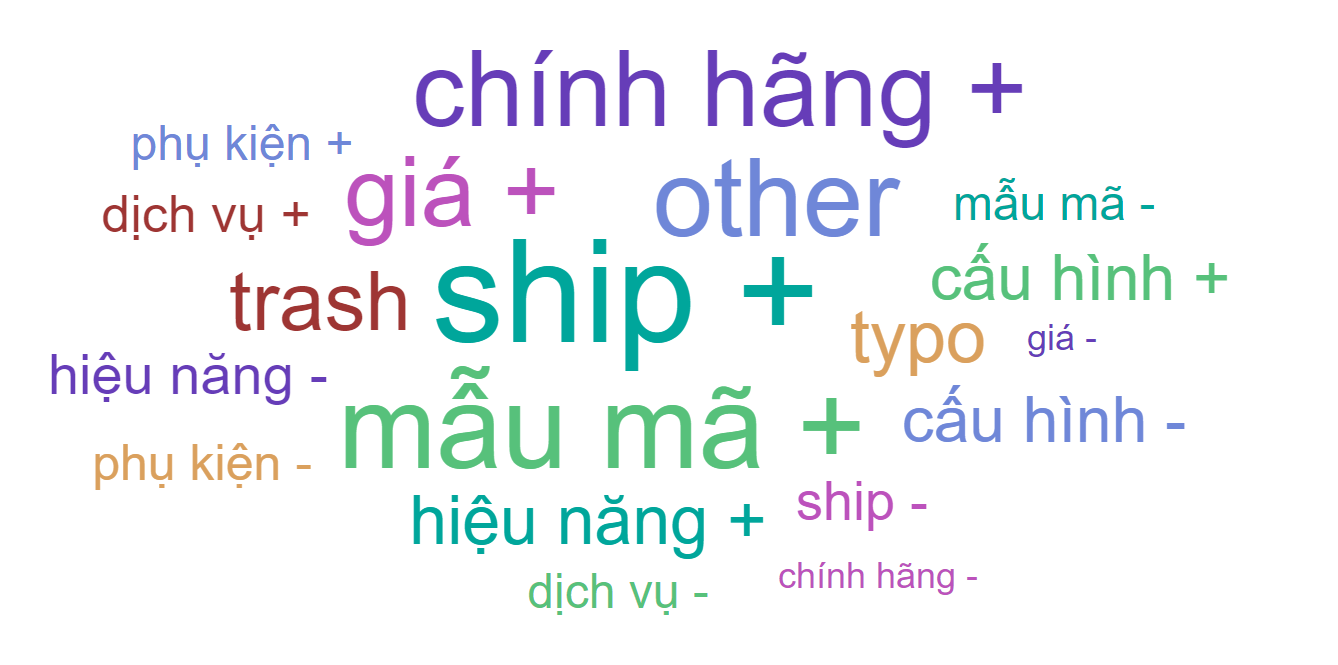
\includegraphics[width=\linewidth]{Chapter4/Figs/kibana1.png}
	\caption{Dataset visualization based on labels and polarity}
	\label{fig:label}
\end{figure}

\begin{figure}[h]
	\centering
	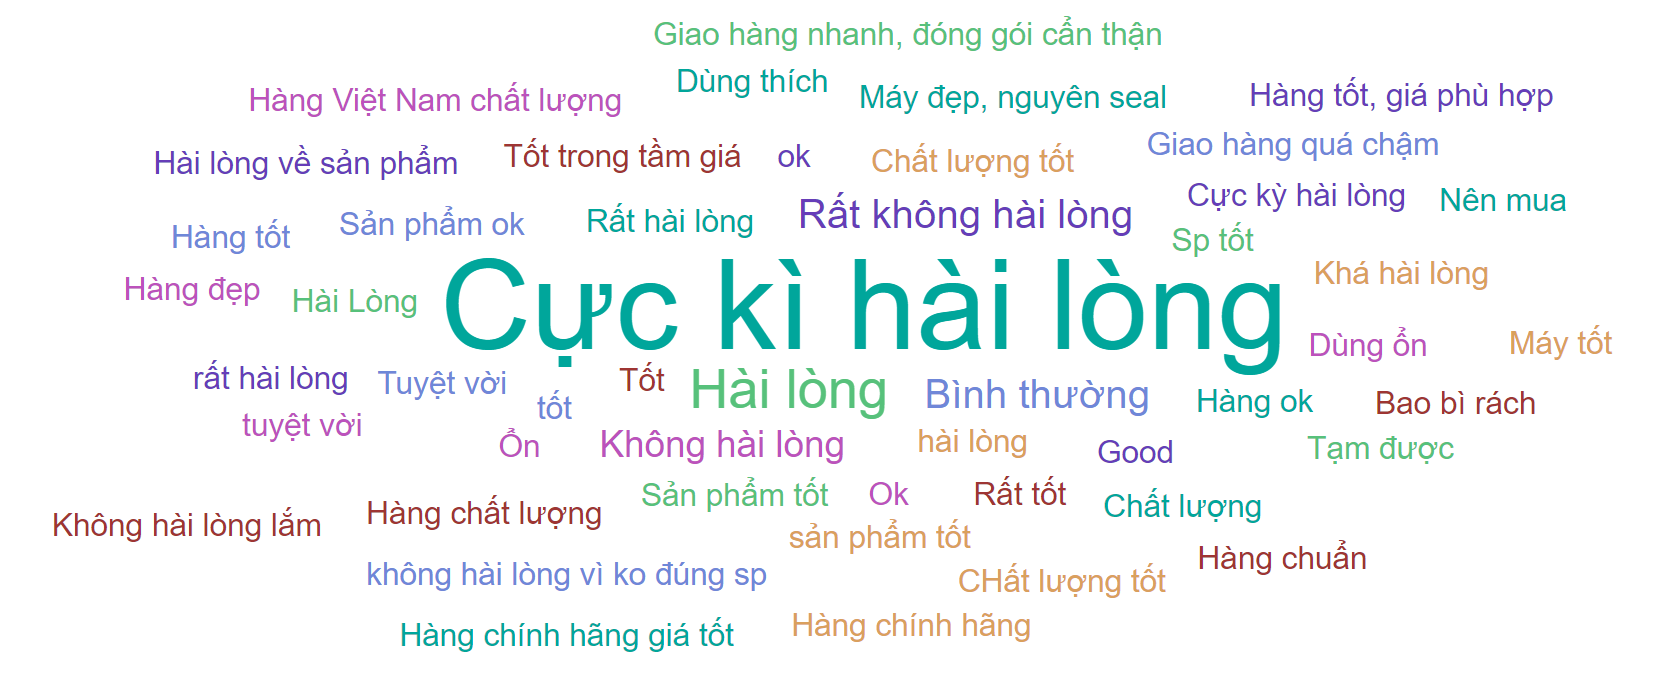
\includegraphics[width=\linewidth]{Chapter4/Figs/kibana2.png}
	\caption{Dataset visualization based on keywords}
	\label{fig:keyword}
\end{figure}

\subsection{Web Application Demonstration}
With a view to bring the model into practical situation, we built a web interface for users to manipulate easily.
The users will put in data in two ways: insert each comment by the 'Add' button (figure~\ref{fig:tool1}) or import a CSV file containing comment data along with the respective aspect (figure~\ref{fig:tool2}).

\begin{figure}[h]
	\centering
	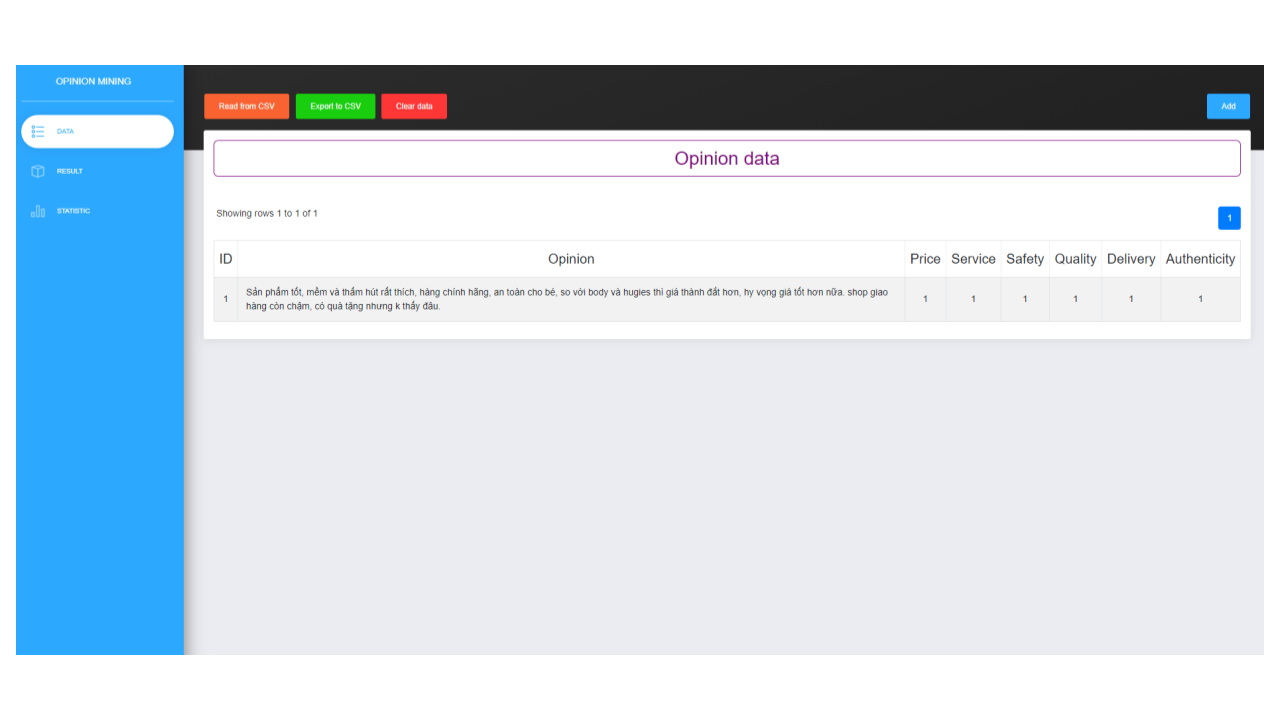
\includegraphics[width=\linewidth]{Chapter4/Figs/tool1.png}
	\caption{Insert comment by the 'Add' button}
	\label{fig:tool1}
\end{figure}

\begin{figure}[h]
	\centering
	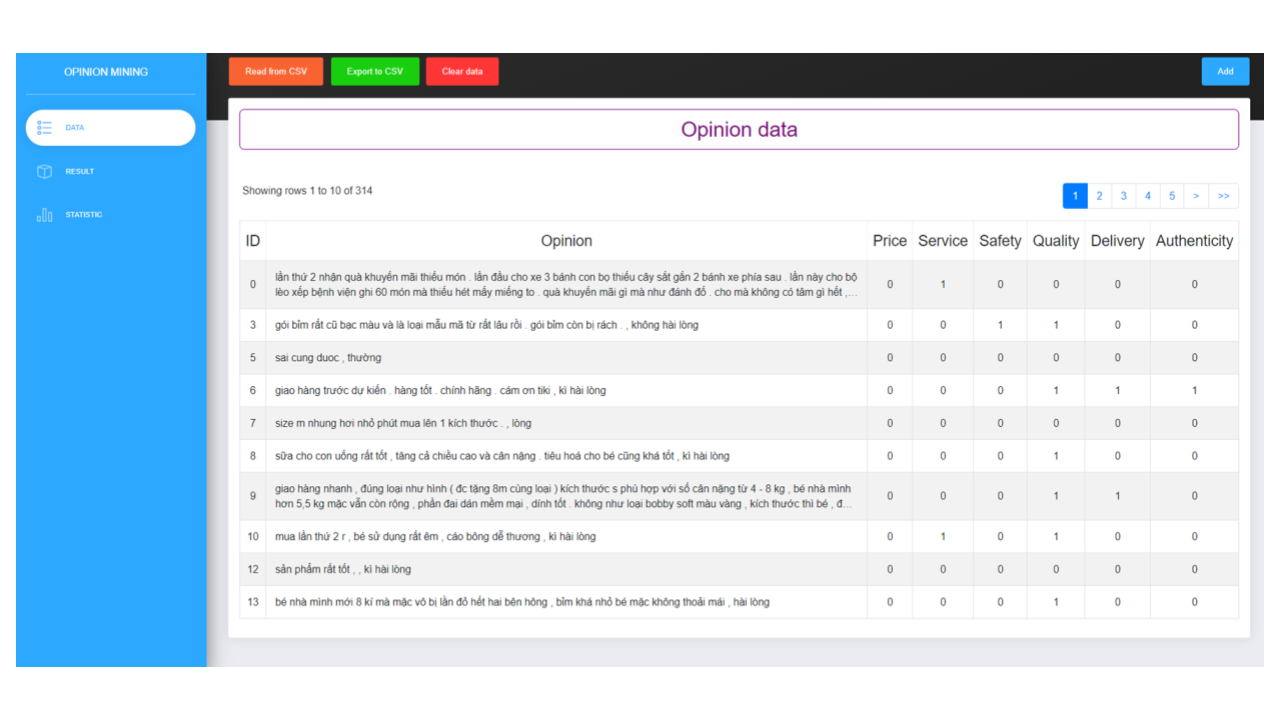
\includegraphics[width=\linewidth]{Chapter4/Figs/tool2.png}
	\caption{Insert comments by importing CSV file}
	\label{fig:tool2}
\end{figure}

The model runs when the user selects 'Result' button. The results as illustrated in figure~\ref{fig:tool3} and~\ref{fig:tool4} show -1 and 1 on the aspects that appear in the comment corresponding to the negative and positive emotions related to that aspect.

\begin{figure}[h]
	\centering
	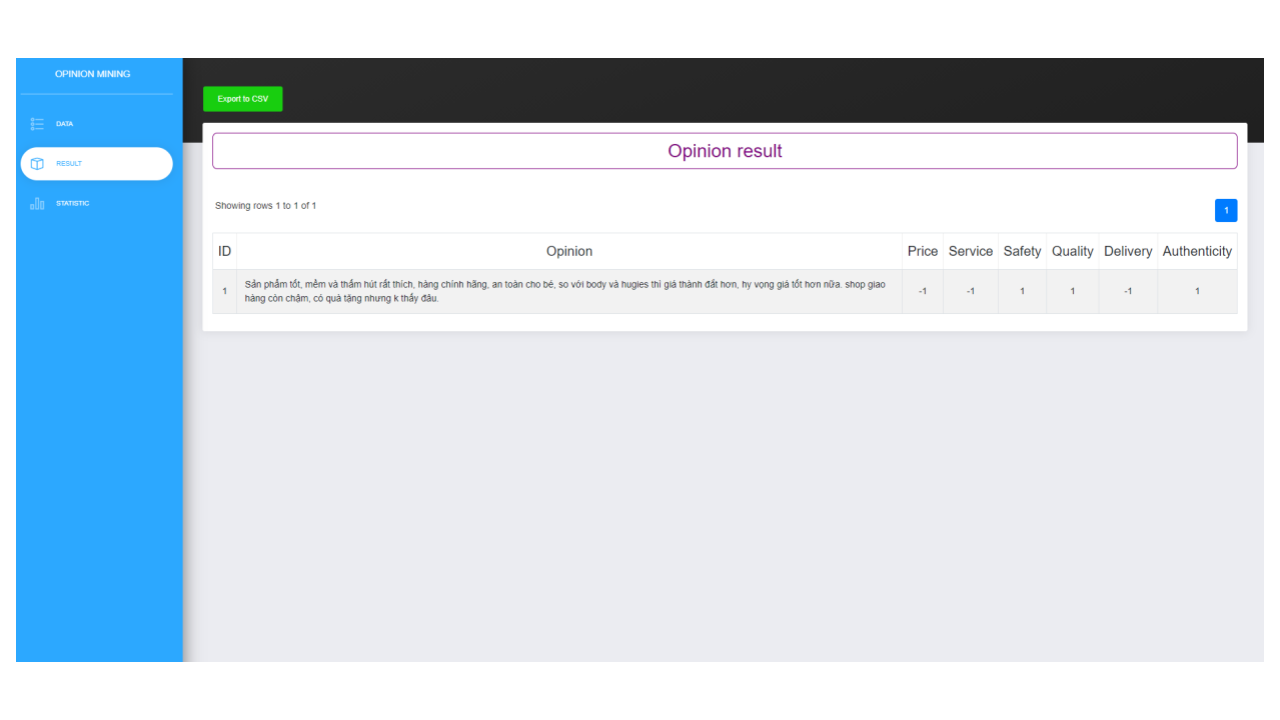
\includegraphics[width=\linewidth]{Chapter4/Figs/tool3.png}
	\caption{Model output when using 'Add" function}
	\label{fig:tool3}
\end{figure}

\begin{figure}[h]
	\centering
	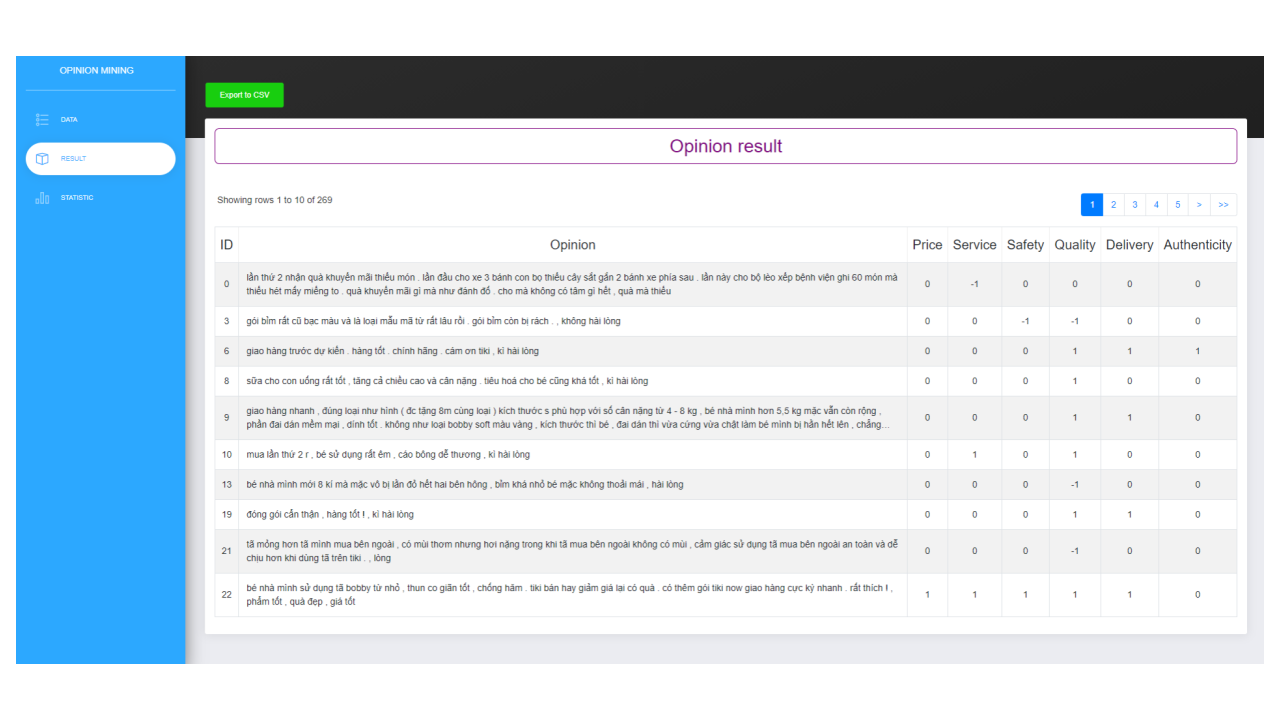
\includegraphics[width=\linewidth]{Chapter4/Figs/tool4.png}
	\caption{Model output when using 'Import" function}
	\label{fig:tool4}
\end{figure}

In addition, we have built a few functions for the web application such as showing detailed statistical results of positive and negative sentiment on each aspects, exporting results in CSV, PNG, etc. formats for data statistics and visualization.

\begin{figure}[h]
	\centering
	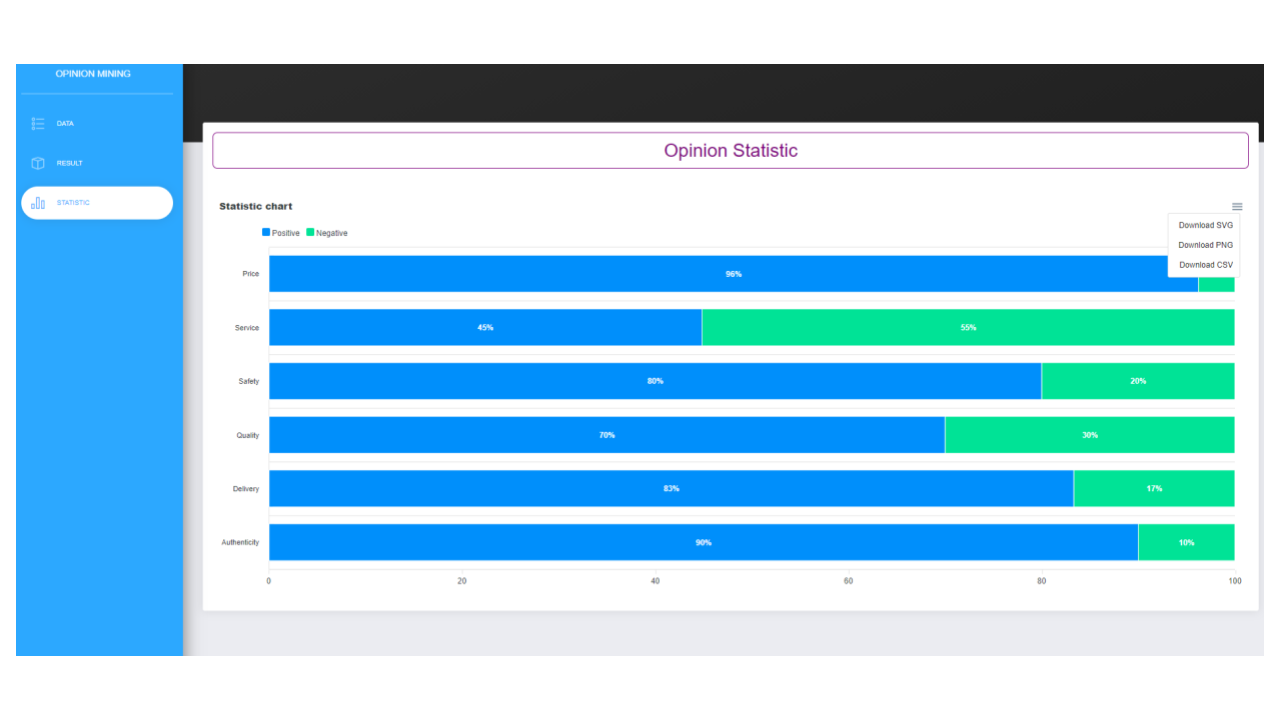
\includegraphics[width=\linewidth]{Chapter4/Figs/tool5.png}
	\caption{Detailed statistical results of positive and negative sentiment on each aspects}
	\label{fig:tool5}
\end{figure}
